\providecommand{\main}{../../../..}
\documentclass[\main/dresen_thesis.tex]{subfiles}
\begin{document}
  \label{sec:colloidalCrystals:vsm}

  \begin{figure}[tb]
    \centering
    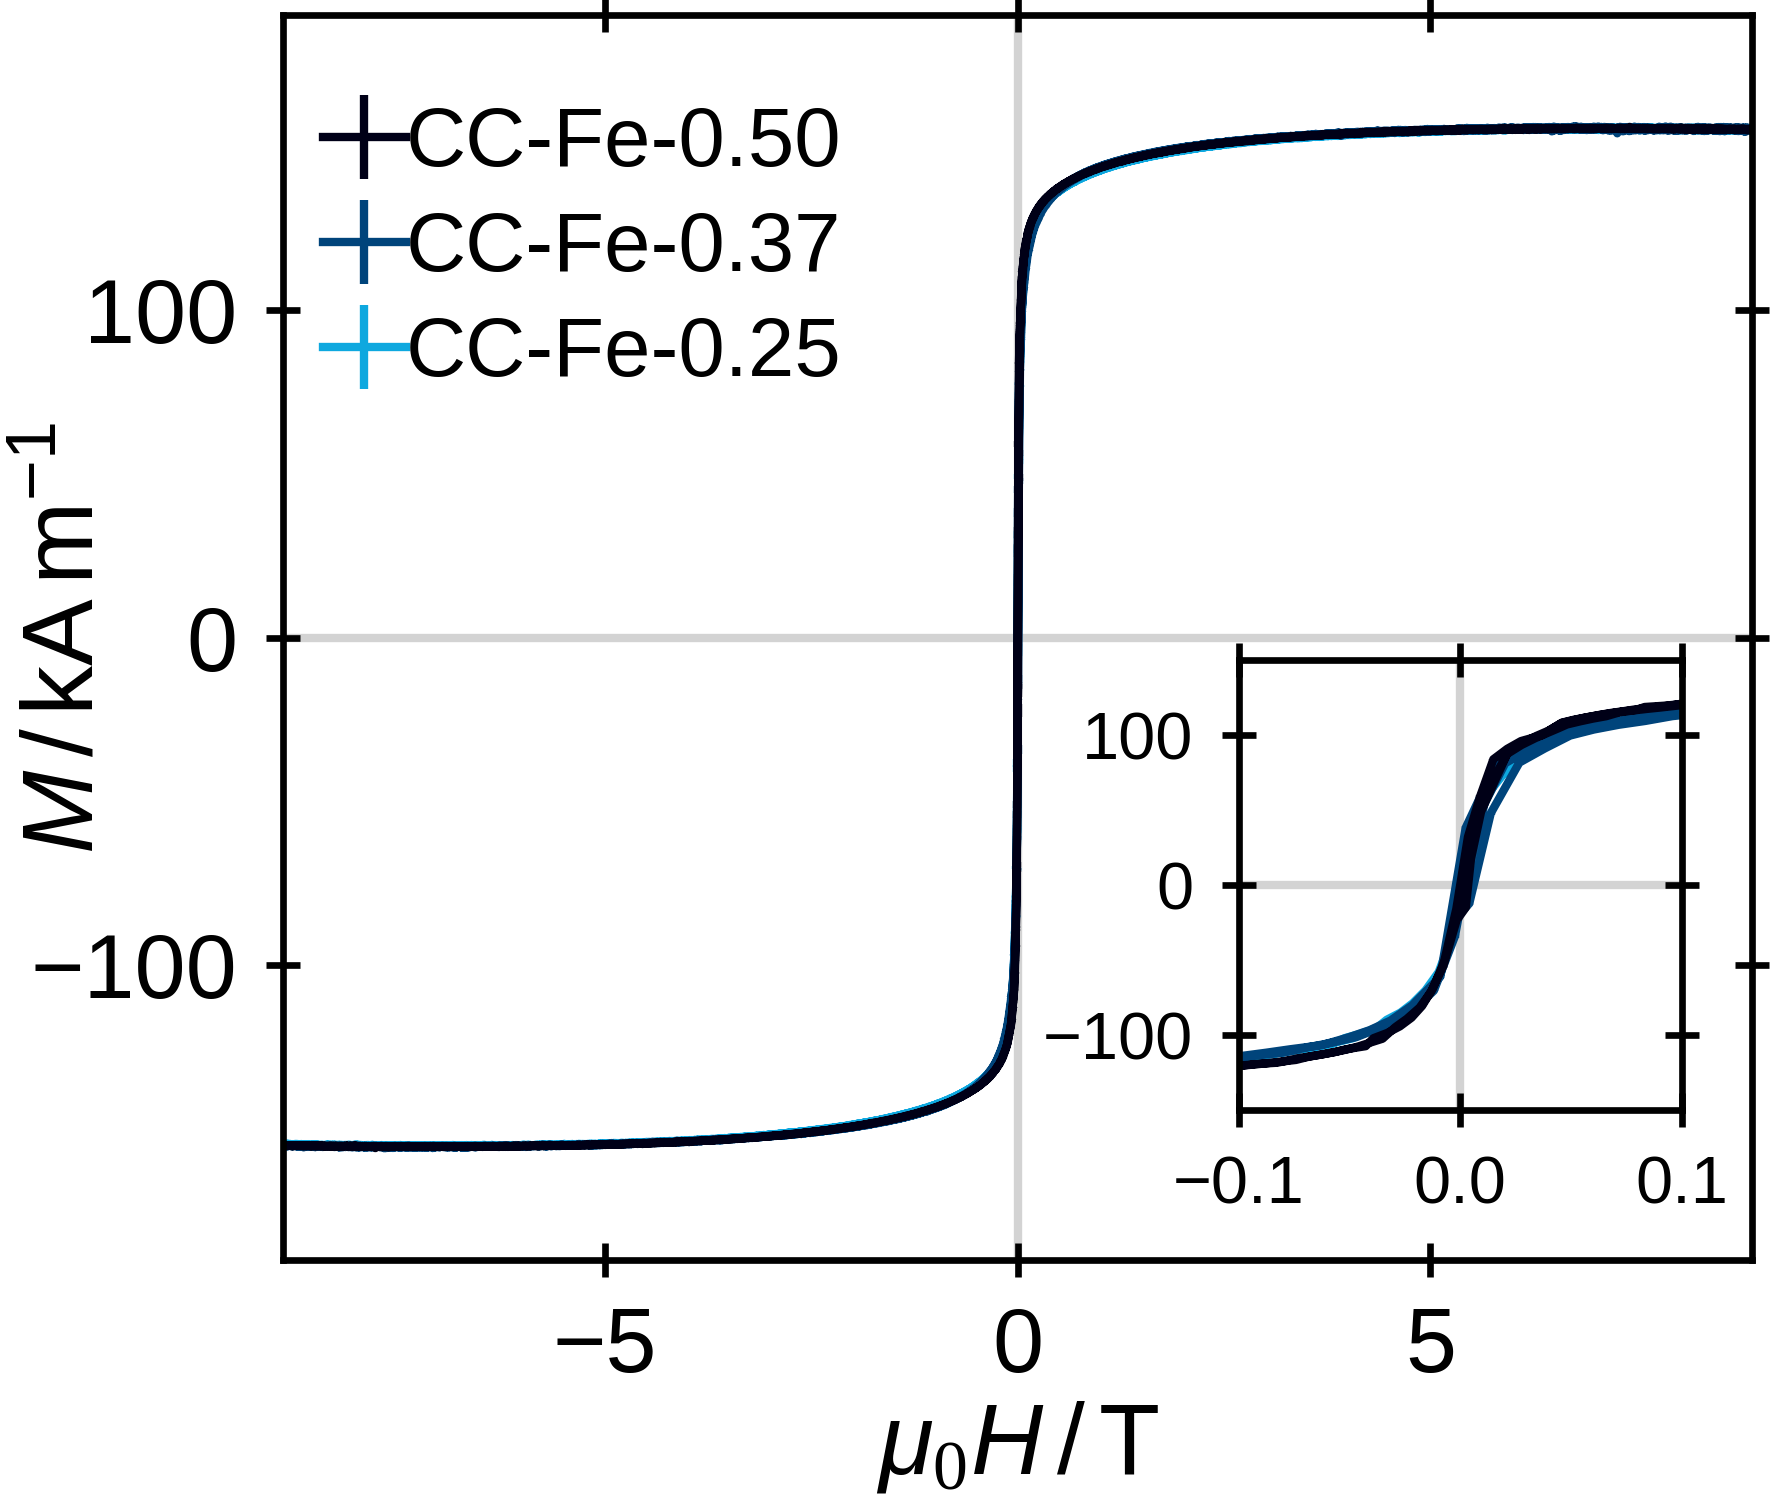
\includegraphics{colloidalCrystals_PPMS_300K_allSamples}
    % 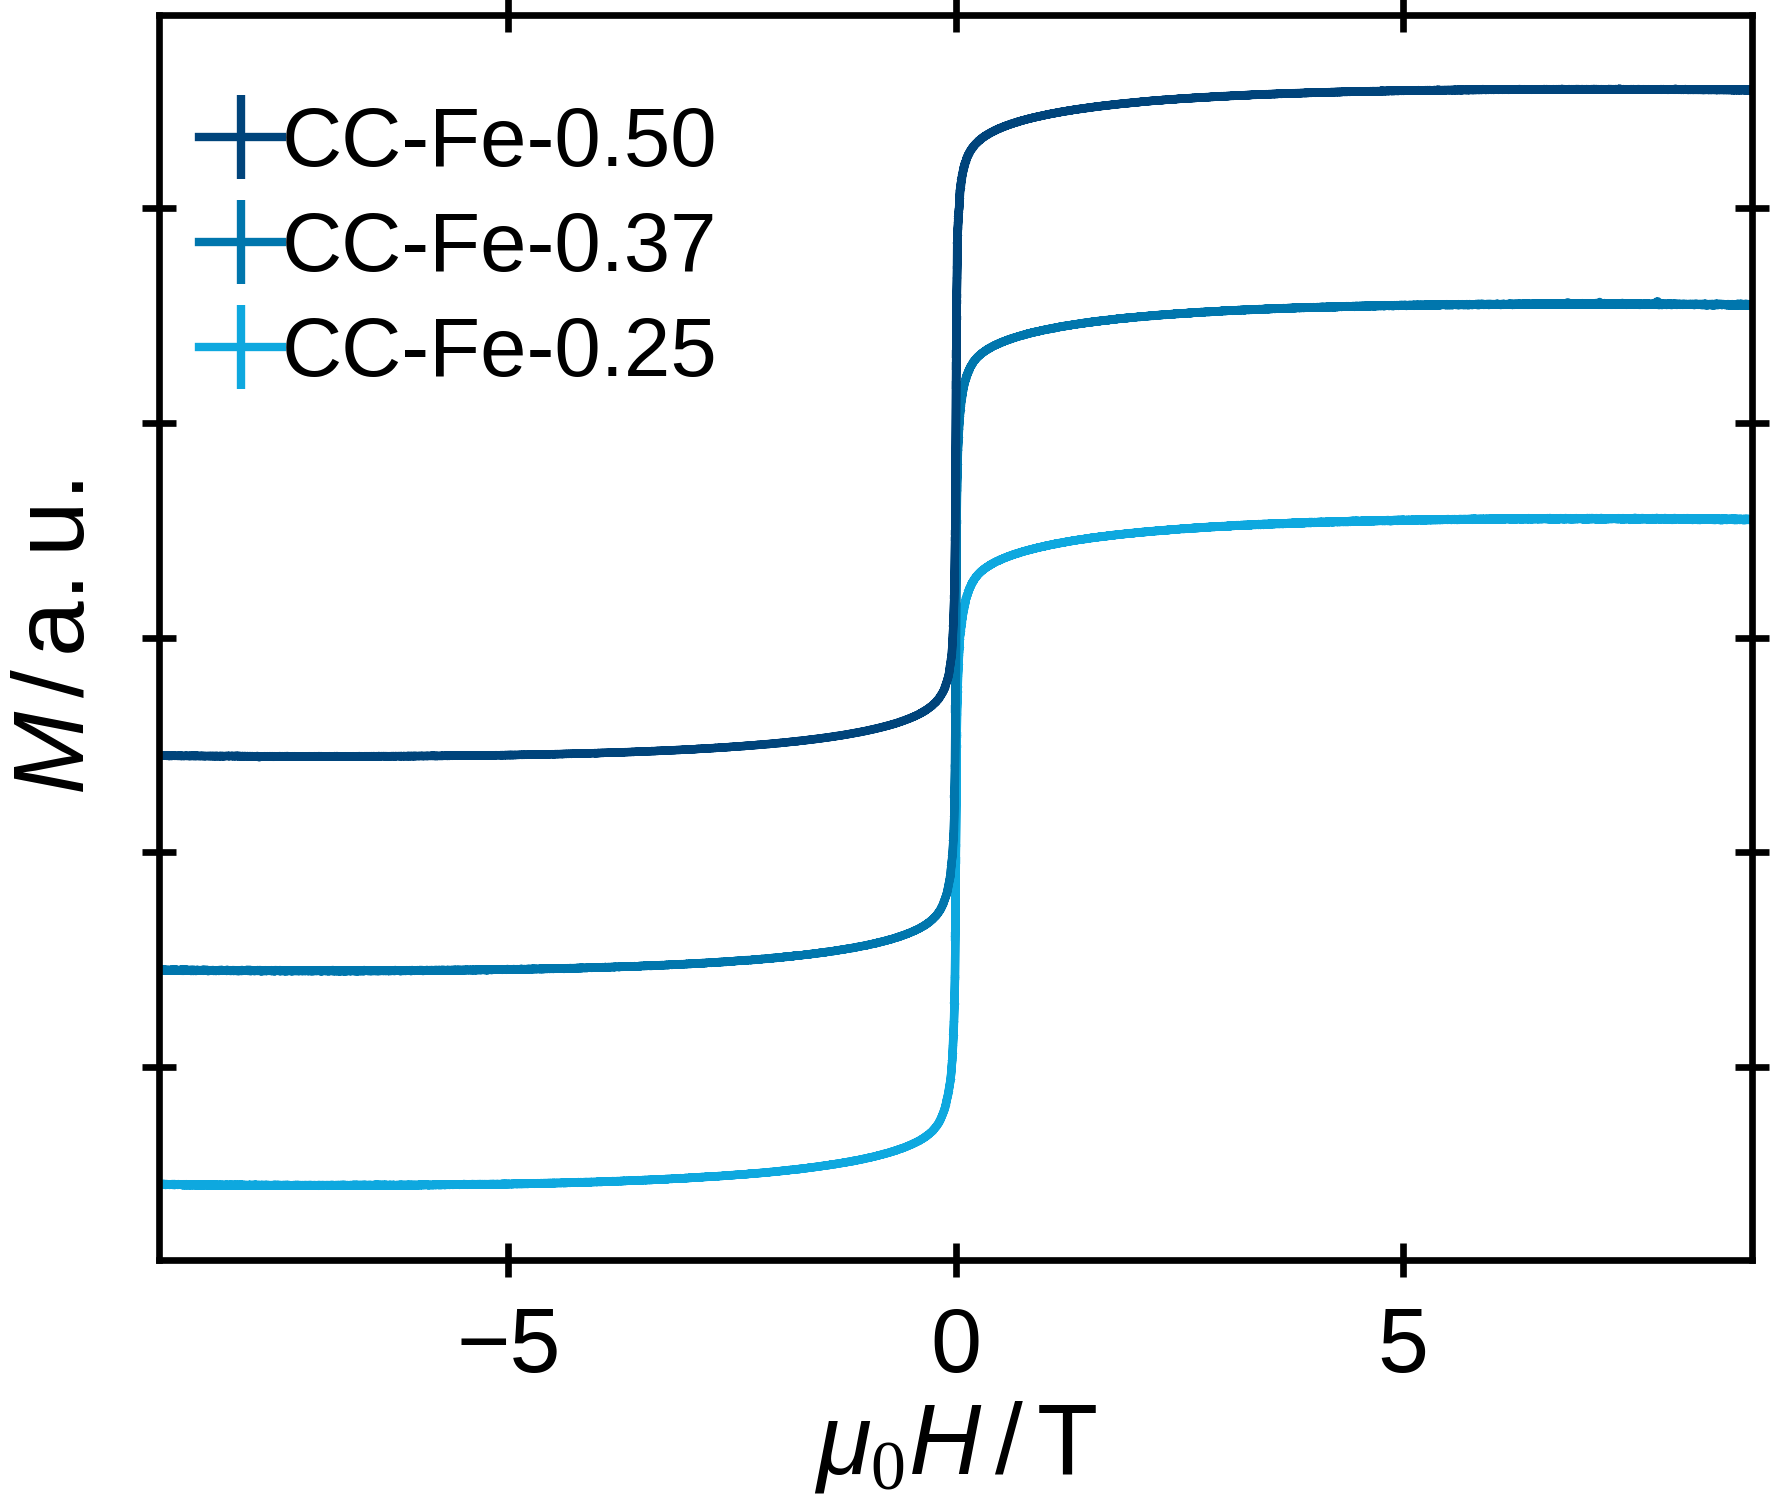
\includegraphics{colloidalCrystals_PPMS_300K_allSamplesShifted}
    \caption{\label{fig:colloidalCrystals:RTVSM}Field-dependent magnetization at $300 \unit{K}$ of the colloidal crystals. The data is corrected for the diamagnetic susceptibility of the background and scaled to the observed spontaneous magnetization given in \reftab{tab:colloidalCrystals:RTVSM:parameters}.}
  \end{figure}

  \paragraphNewLine{Room temperature magnetization}
    In a first step the colloidal crystals are measured on the PPMS Evercool II at room temperature to determine the spontaneous magnetization and susceptibility at high fields.
    By performing a linear fit between $5 - 9 \unit{T}$, the two values are obtained as tabulated in \reftab{tab:colloidalCrystals:RTVSM:parameters}.

    \begin{table}[!htbp]
      \centering
      \caption{\label{tab:colloidalCrystals:RTVSM:parameters} Spontaneous magnetization $M_s$ and susceptibility $\chi$ of the raw double layer magnetization determined by fitting the slope of the data in the range of $5 - 9 \unit{T}$. As well as scaled to the mass of the silicon substrate and therefore to the measured sample area.}
      \begin{tabular}{ l | l | l || l | l}
        \rule{0pt}{2ex} \textbf{VSM @ 300 K}
        & $M_s \, / \unit{memu}$
        & $\chi \, / \unit{\musf emu \, T ^{-1}}$
        & $\bar{M}_s \, / \unit{memu / g}$
        & $\bar{\chi} \, / \unit{memu \, T ^{-1} g^{-1}}$ \\
        \hline
        \rule{0pt}{2ex} CC-Fe-0.25    & $1.8480(4)$   & $-16.18(6)$ & $60.25(1)$  & $-0.528(2)$\\
        \rule{0pt}{2ex} CC-Fe-0.37    & $1.5599(5)$   & $-5.46(7)$  & $89.09(3)$  & $-0.312(4)$\\
        \rule{0pt}{2ex} CC-Fe-0.50    & $4.4333(7)$   & $6.68(9)$   & $126.30(2)$ & $0.190(3)$\\
        \hline
      \end{tabular}
    \end{table}

    After scaling the observed values to the mass of the wafer and therefore obtaining the magnetizations scaled with respect to the measured wafer surface, it can be seen that the obtained spontaneous magnetization $\bar{M}_s$ is directly correlated to the used concentration of nanocubes in the sample preparation.
    While one might possibly expect this, it is in discrepancy with the observation made by scanning electron microscopy in \refsec{sec:colloidalCrystals:layers:sem}, where a non-linear relation between the sample thickness and the used particle concentration is seen.
    To have both observations have in agreement with each other, this means that the seen holes in the colloidal crystals have to make up for the difference.
    Such that even though thicker areas of the sample were observed by cross-sectional SEM micrographs, on average the amount of nanocubes distributed on the wafer is lower than would be expected from the SEM micrograph alone.

    The susceptibility of the curves is relatively small in direct comparison to the sample magnetization but tends to increase with the amount of nanocubes on the wafer.
    This is connected to the paramagnetic phase in the nanocube cores, which provides a positive paramagnetic contributions that increases with the sample amount on the substrate.
    The observed susceptibility is then a combination of the samples paramagnetism and the substrates diamagnetism.

    Correcting the measured magnetism for the varying susceptibility and scaling the spontaneous magnetization to the value observed from the dry powder of nanocubes in \refsec{sec:colloidalCrystals:nanoparticle:vsm}, \reffig{fig:colloidalCrystals:RTVSM} shows that the three magnetization behaviors exactly match with one another.

  \paragraphNewLine{Temperature-dependent magnetization}

    \begin{figure}[tb]
      \centering
      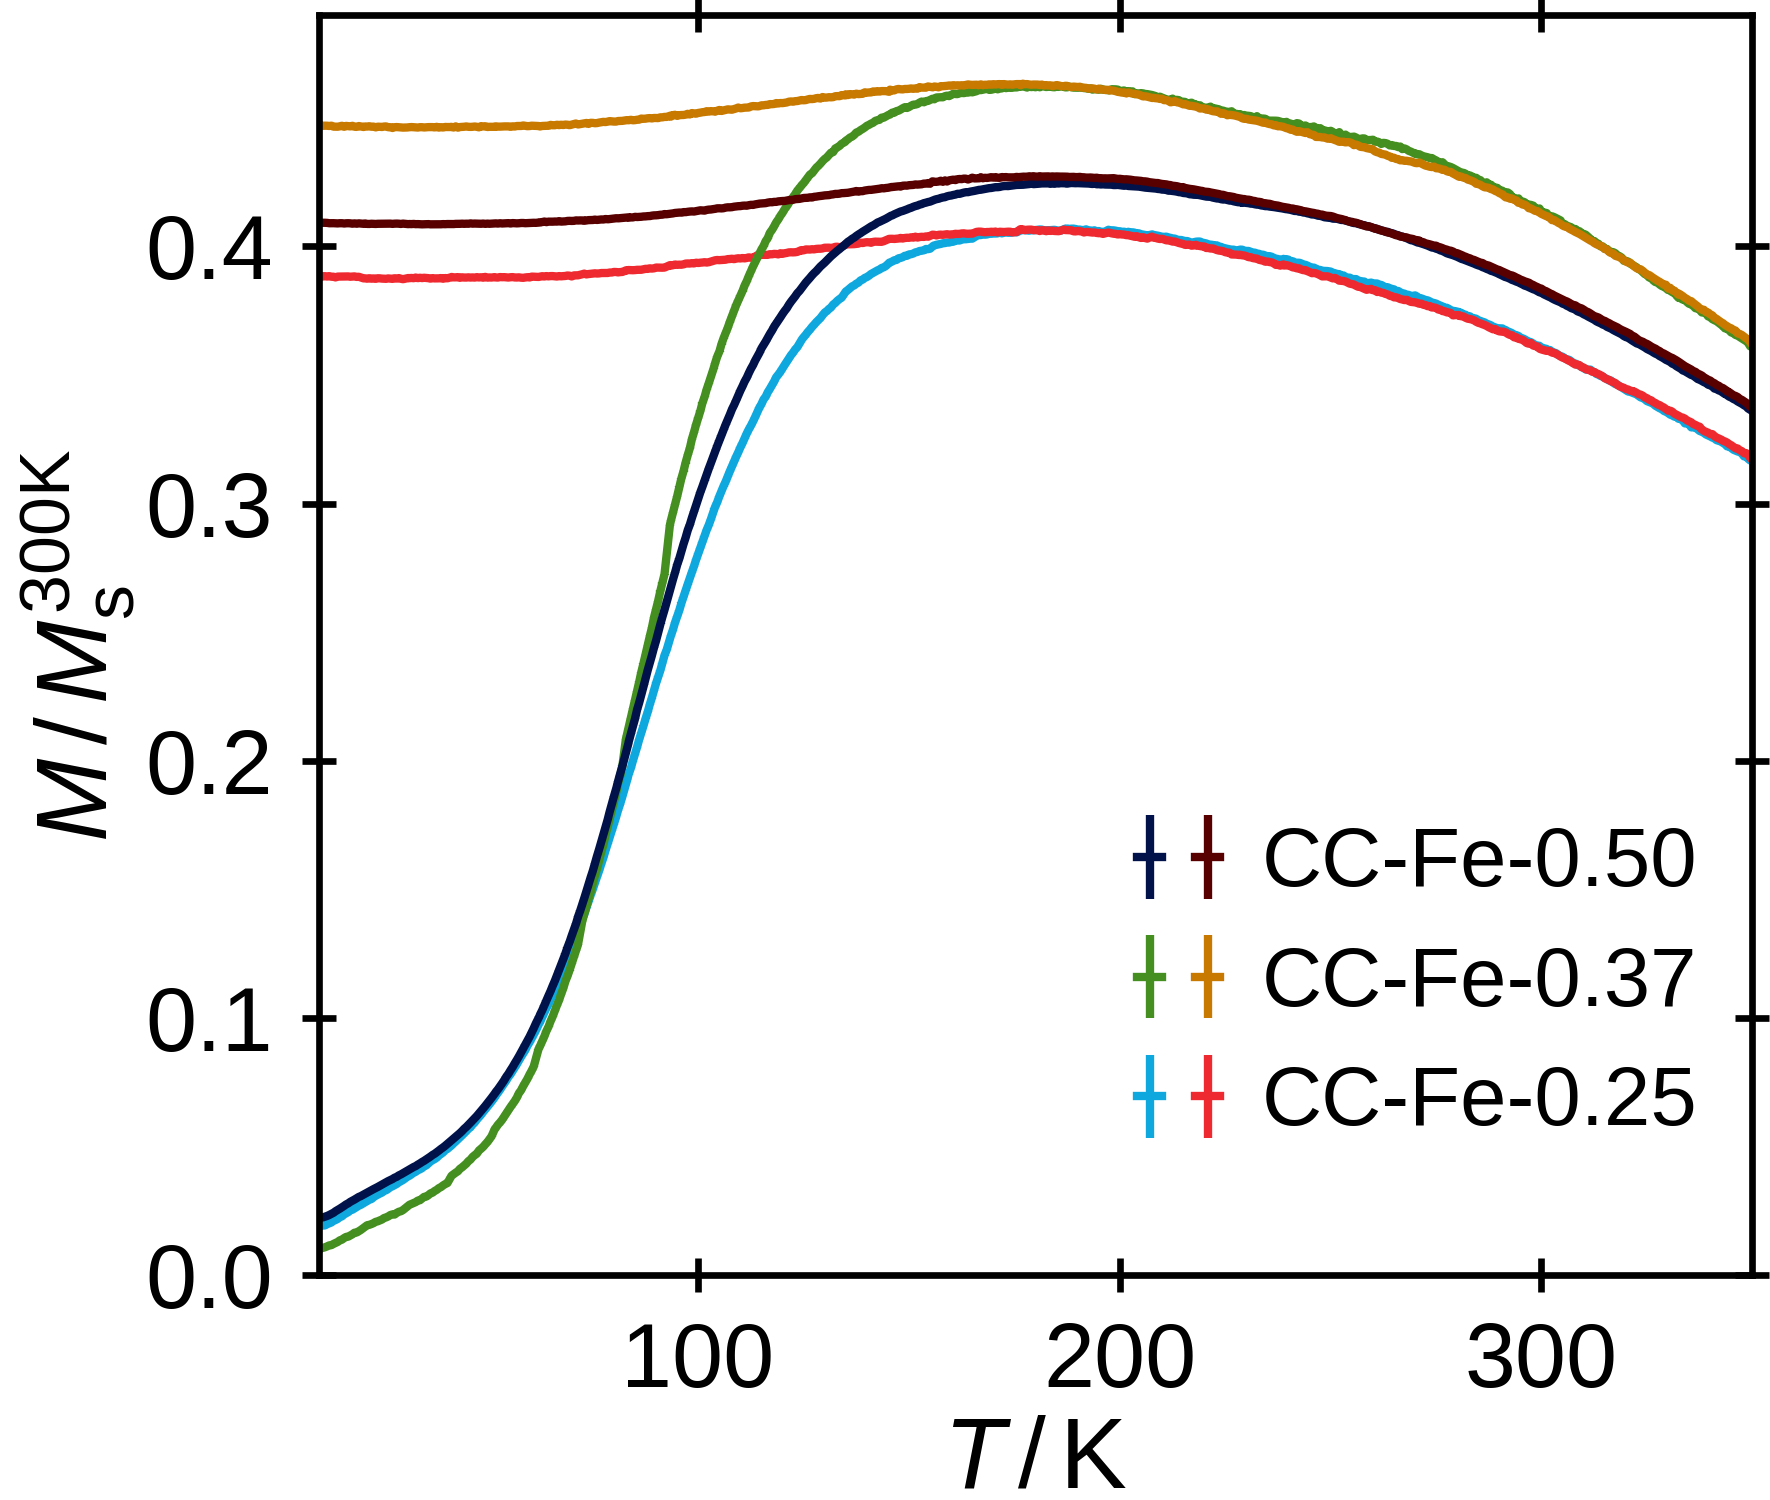
\includegraphics{colloidalCrystals_PPMS_ZFC_FC_allSamples}
      \caption{\label{fig:colloidalCrystals:zfcFCData}Zero-field cooled (red) and field cooled (blue) magnetizations of the three colloidal crystals. The ZFC/FC magnetizations are taken with a field of $10 \unit{mT}$ while warming the sample.}
    \end{figure}

    \begin{table}[!htbp]
      \centering
      \caption{\label{tab:colloidalCrystals:ZFCFC:parameters} Temperatures of the peaks observed in the zero-field and field cooled magnetization of the colloidal crystals shown in \reffig{fig:colloidalCrystals:zfcFCData}.}
      \begin{tabular}{ l | l | l}
        \rule{0pt}{2ex} \textbf{ZFC/FC @ 10 mT}
        & $T_p^\mathrm{ZFCw} \, / \unit{K}$
        & $T_p^\mathrm{FCw} \, / \unit{K}$\\
        \hline
        \rule{0pt}{2ex} CC-Fe-0.25    & $187(1)$   & $181(1)$\\
        \rule{0pt}{2ex} CC-Fe-0.37    & $182(1)$   & $172(1)$\\
        \rule{0pt}{2ex} CC-Fe-0.50    & $187(1)$   & $181(1)$\\
        \hline
      \end{tabular}
    \end{table}

    For the colloidal crystals, the zero-field and field cooled magnetization is measured at a field of $10 \unit{mT}$ and shown in \reffig{fig:colloidalCrystals:zfcFCData}.
    The rescaling of the data was performed as determined from the spontaneous magnetization at room temperature.
    In each case a peak can be observed in both the field cooled and zero-field cooled curve, where the positions for the three samples is determined as tabulated in \reftab{tab:colloidalCrystals:ZFCFC:parameters}.
    It is visible that the temperatures of CC-Fe-0.37, are significantly shifted by $5 \unit{K}$ in the ZFC data and $9 \unit{K}$ in the FC data towards smaller temperatures than observed for CC-Fe-0.25 and CC-Fe-0.50, where the same peak values are observed.
    From SEM, the intermediate sample CC-Fe-0.25 was considered the sample with the best structural order among the three, which might show it's manifestation at this point.
    As dipolar interaction among the nanoparticles is a long-ranged interaction, the higher structure allows for a stronger collective interaction of the sample.
    As the sample is warmed, less thermal energy is then needed to overcome the magnetocrystalline barrier as the sample

  \paragraphNewLine{Field-dependent low temperature magnetization}

    \begin{figure}[tb]
      \centering
      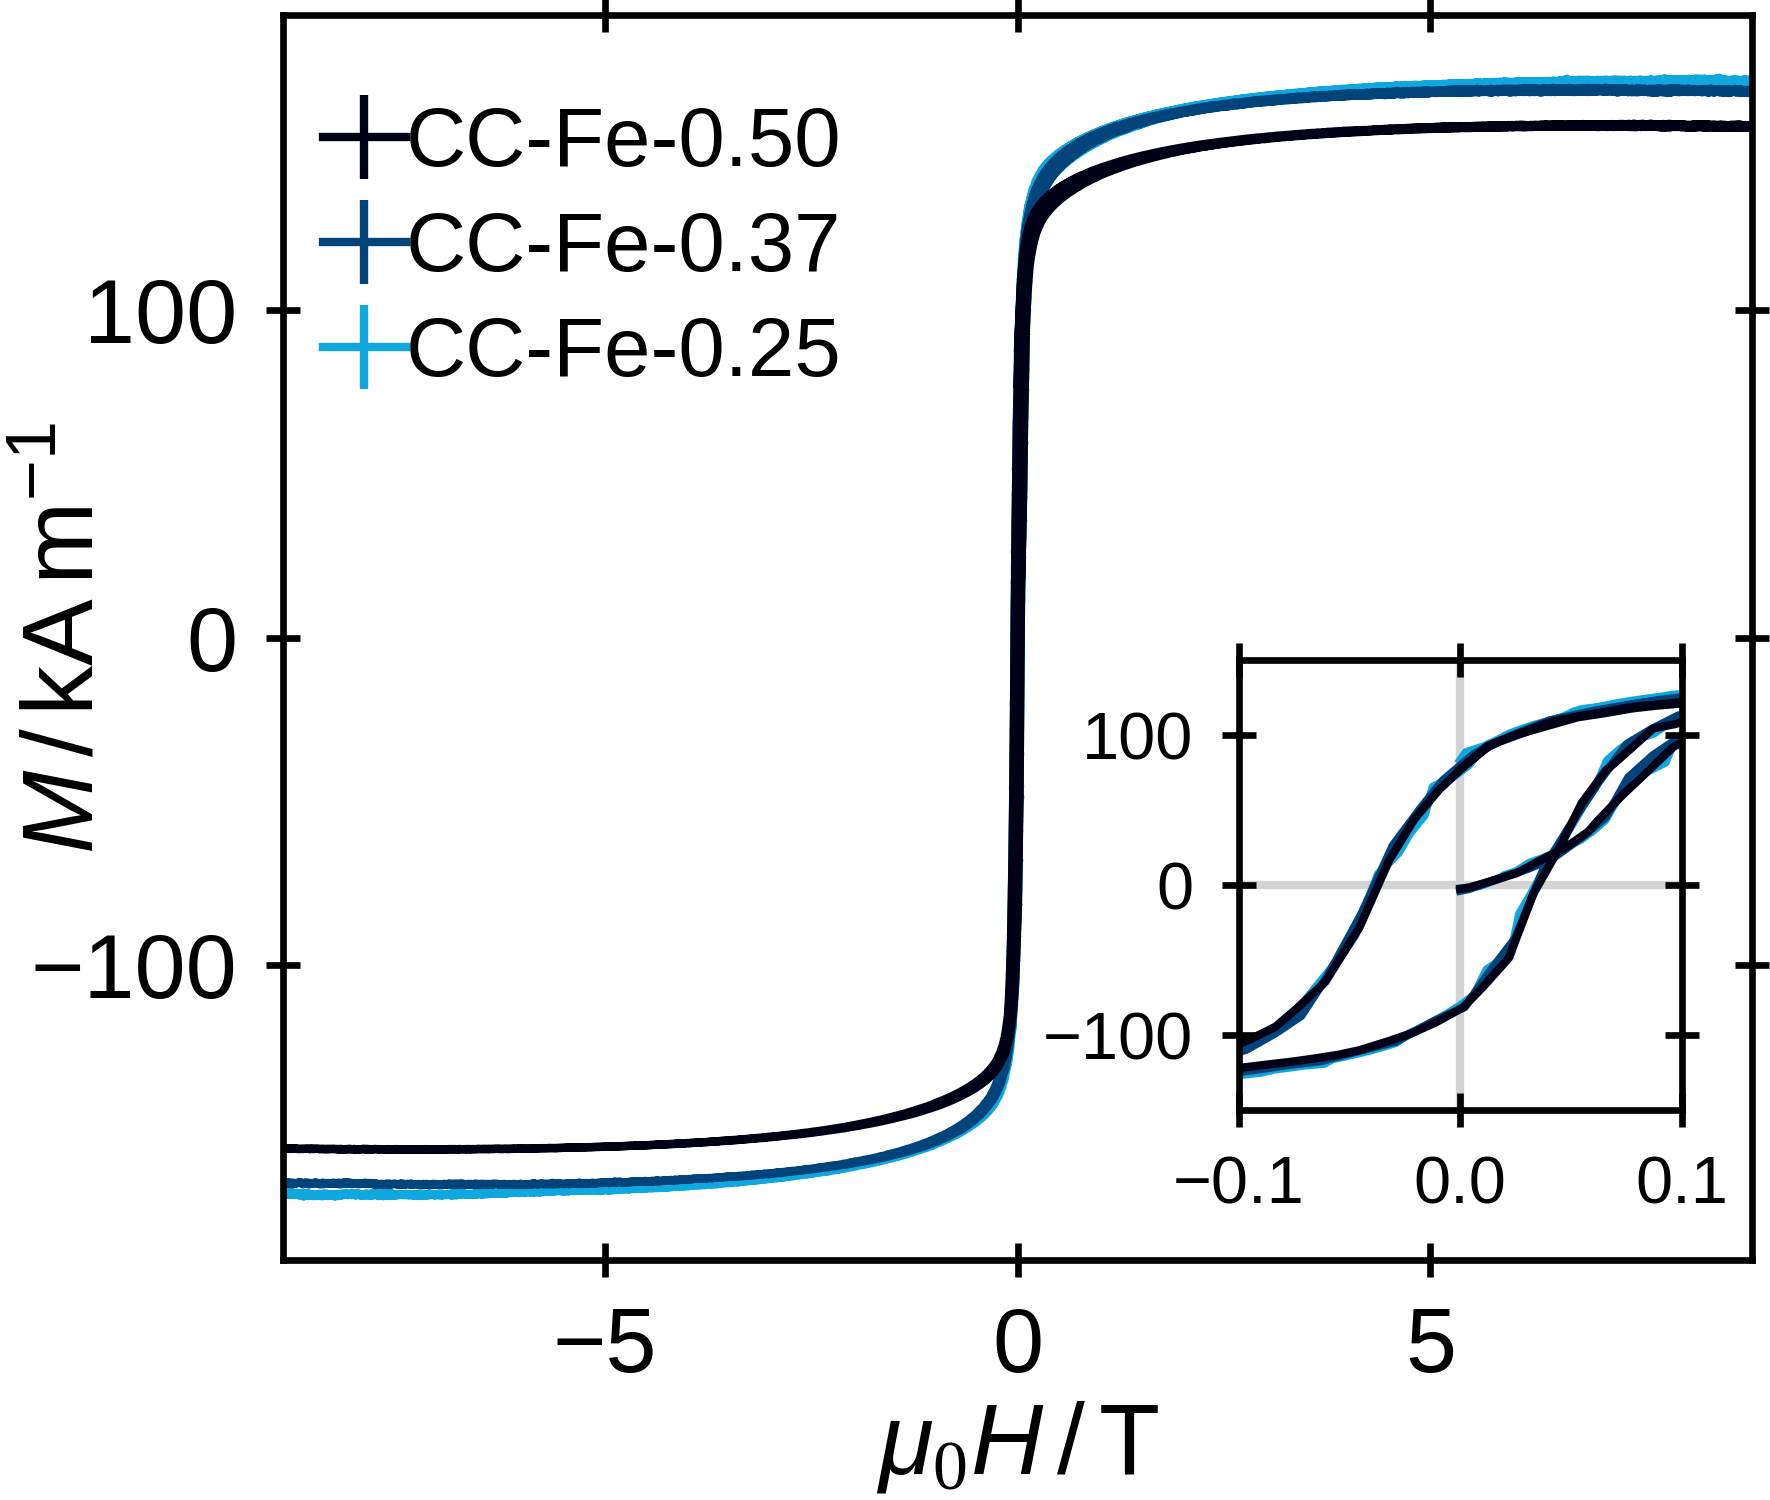
\includegraphics{colloidalCrystals_PPMS_10K_allSamples}
      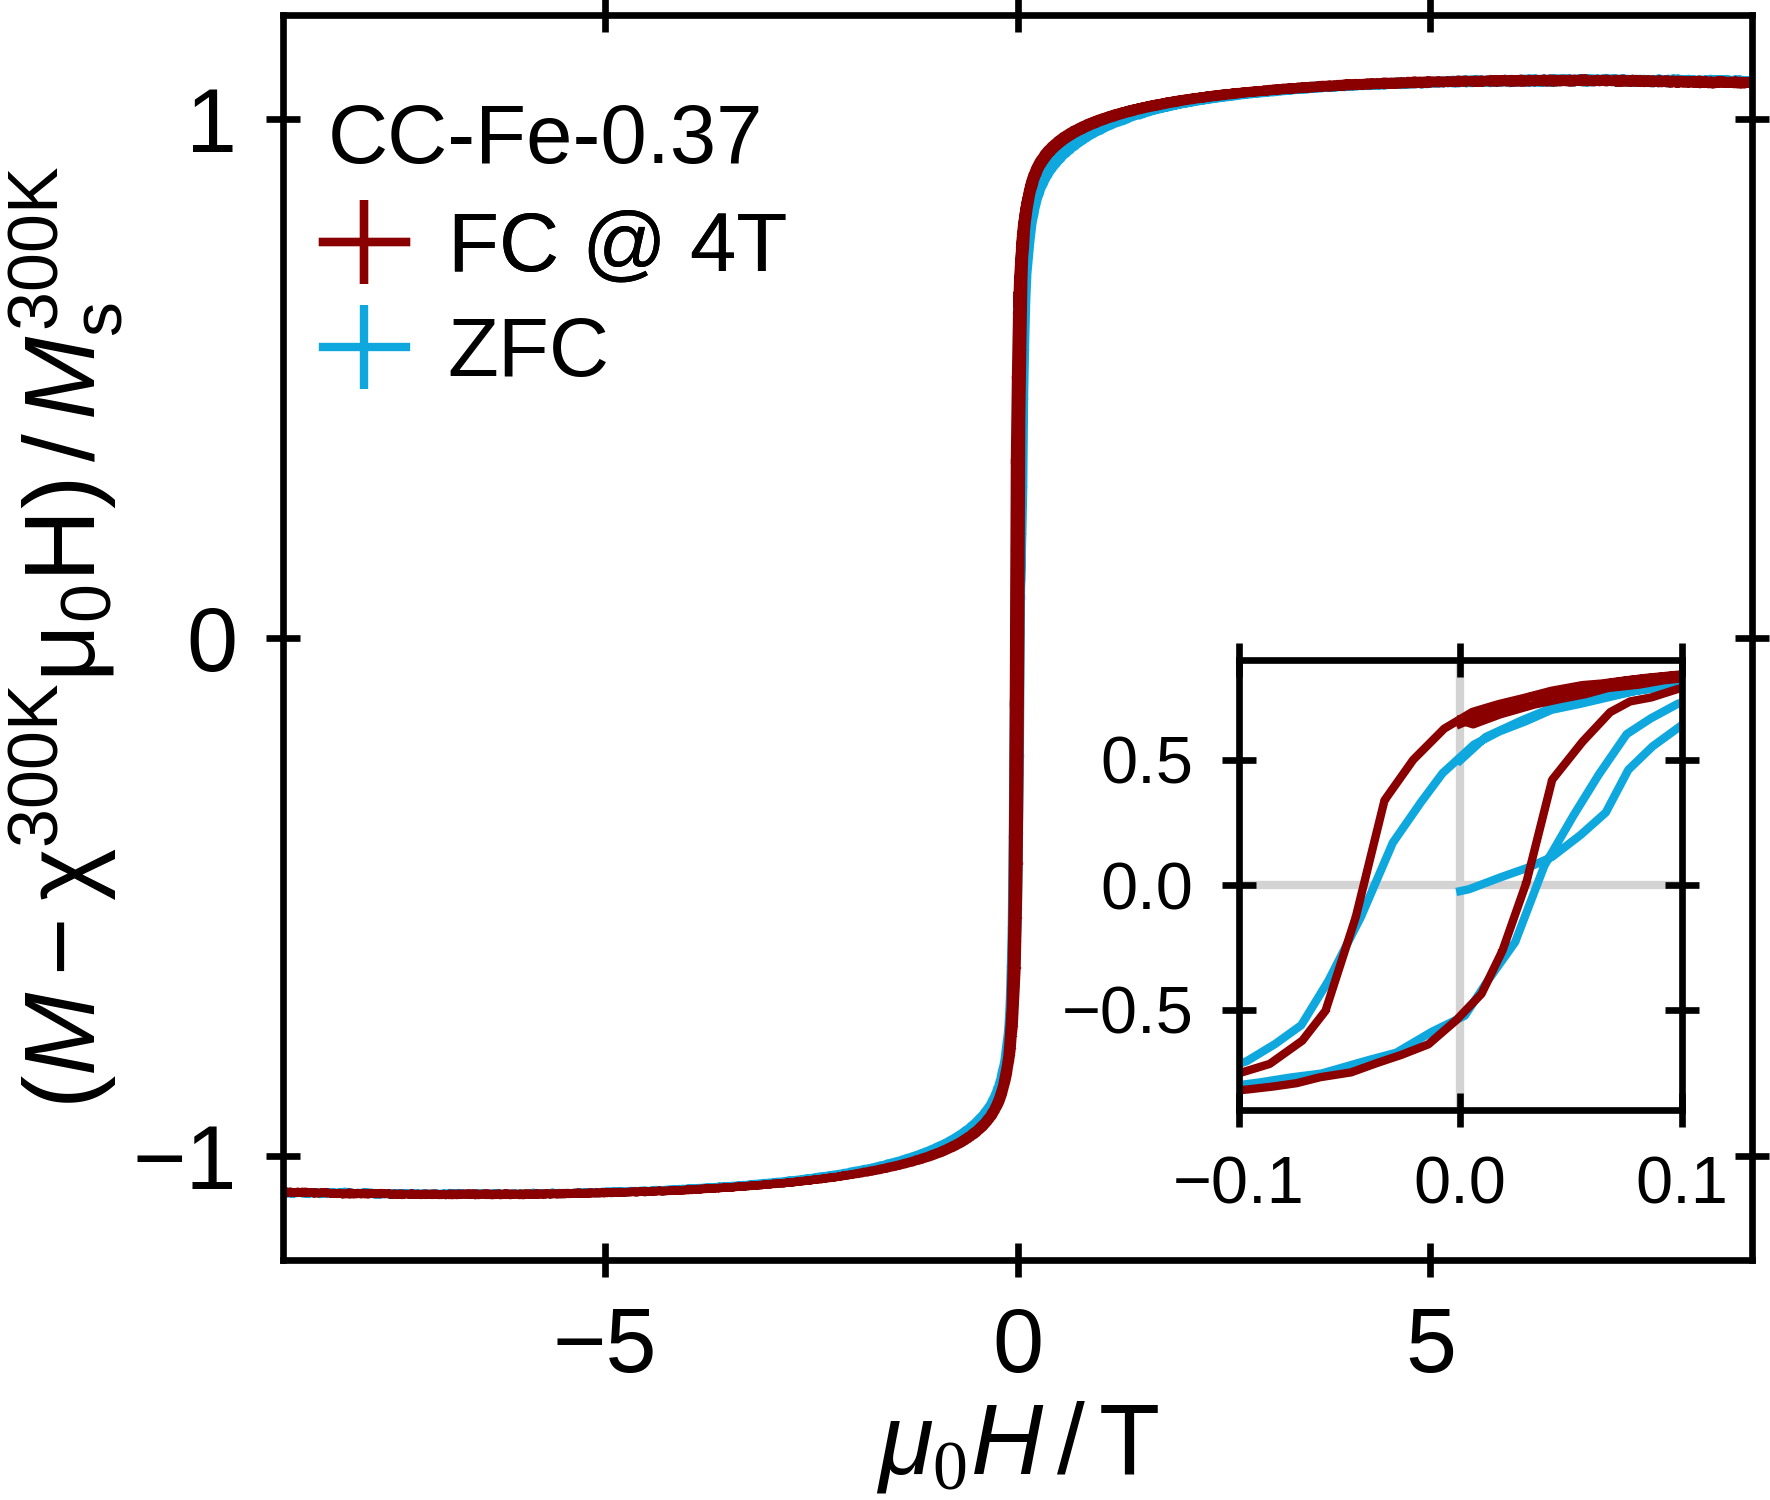
\includegraphics{colloidalCrystals_PPMS_10K_CC-Fe-0-37_EB}
      \caption{\label{fig:colloidalCrystals:10KVSM}Low temperature field-dependent magnetization of the colloidal crystals measured at $10 \unit{K}$. The colloidal crystals are all measured after zero-field cooling (left). Furthermore, the effect of field cooling the sample in a strong magnetic field of $4 \unit{T}$ on the hysteresis is shown for CC-Fe-0.37 (right).}
    \end{figure}
    The samples CC-Fe-0.25, CC-Fe-0.37 and CC-Fe-0.50 were both measured field-dependent at $10 \unit{K}$ after zero-field cooling. The data is rescaled as determined by the room temperature measurement and shown in \reffig{fig:colloidalCrystals:10KVSM}.
    It can be seen that at low magnetic fields, a close match in the coercive field is given, which is observed to be $35(1) \unit{mT}$.
    At larger fields the curves separate however and the thin sample CC-Fe-0.25 reaches a higher spontaneous magnetization in comparison to the thicker samples, where the lowest saturation value is observed for the CC-Fe-0.50 sample.
    Furthermore, it is studied which effect the application of a magnetic field during the cool down has on the example of the magnetization of CC-Fe-0.37.
    After cooling in a $4 \unit{T}$ field, a negative exchange-bias shift in the order of $5(1) \unit{mT}$ can be seen, as well as an increase of the remanent magnetization by $25 \%$.
    The saturating magnetization of the sample is otherwise analogue to the zero-field cooled hysteresis.
    The exchange-bias effect is connected to the core-shell structure of the iron cubes as it is also commonly observed in literature for iron oxide nanocubes prepared from iron oleates \cite{Wetterskog_2013_Anoma}.
\end{document}